%----------------------------------------------------------------------------
\chapter{\bevezetes}
%----------------------------------------------------------------------------
A vezetés számomra mindig többet jelentett egyszerű feladatkiosztásnál vagy projektirányításnál. 
2019 óta vezető beosztásban dolgozom hangmérnökként és projektmenedzserként egy rendezvénytechnikával foglalkozó cégnél, 
ahol nap mint nap emberekkel, határidőkkel és váratlan helyzetekkel kell egyensúlyt teremtenem. 
Az elmúlt évek során megtapasztaltam, hogy a vezetői szerep nemcsak szakmai tudást, hanem komoly önismeretet, 
kommunikációs készséget és felelősségvállalást is igényel. 

E dolgozat célja, hogy a „Mitől leszek jó vezető?” kérdésre a saját tapasztalataimon és a 84 elemű önértékelő 
teszten alapuló elemzésen keresztül keressem a választ. A téma azért különösen fontos számomra, mert a vezetői 
hatékonyság nemcsak a csapat teljesítményét, hanem a munkakörnyezet hangulatát és a projektek sikerességét is meghatározza.

A dolgozat során először bemutatom a vezetés és a kompetenciák elméleti hátterét, majd a saját szakmai pályámon 
keresztül végzem el a személyes kompetenciaelemzést. Ezt követően részletes fejlesztési tervet készítek a 
fejlesztendő területek erősítésére. A célom, hogy az elemzés segítségével tudatosabban építsem tovább vezetői 
készségeimet, és olyan önfejlesztési irányokat határozzak meg, 
amelyek hozzájárulnak a hosszú távú szakmai és személyes fejlődésemhez.

%----------------------------------------------------------------------------
\begin{figure}[H]
	\centering
	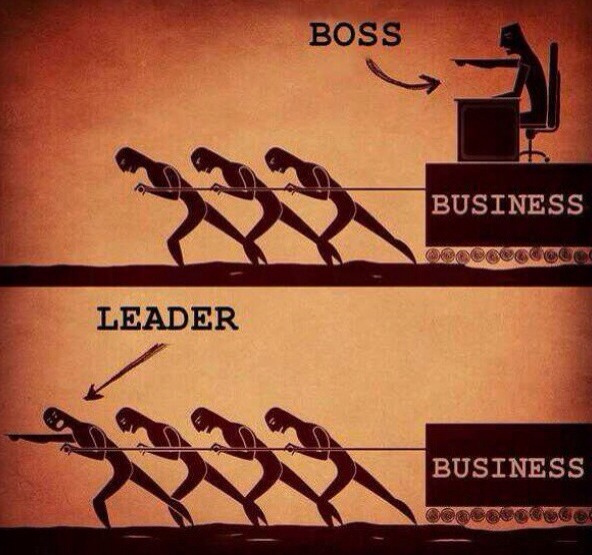
\includegraphics[width=50mm, keepaspectratio]{figures/boss_leader.jpg}
	\caption{A vezető és a főnök közötti különbség illusztrációja}
	\label {fig:boss_leader}
\end{figure}
%----------------------------------------------------------------------------